\section{Question}

\subsection{Select four orthologues, and create a rooted phylogenetic tree using the UPGMA algorithm as shown in class.}

\begin{figure}[ht]
    \centering
    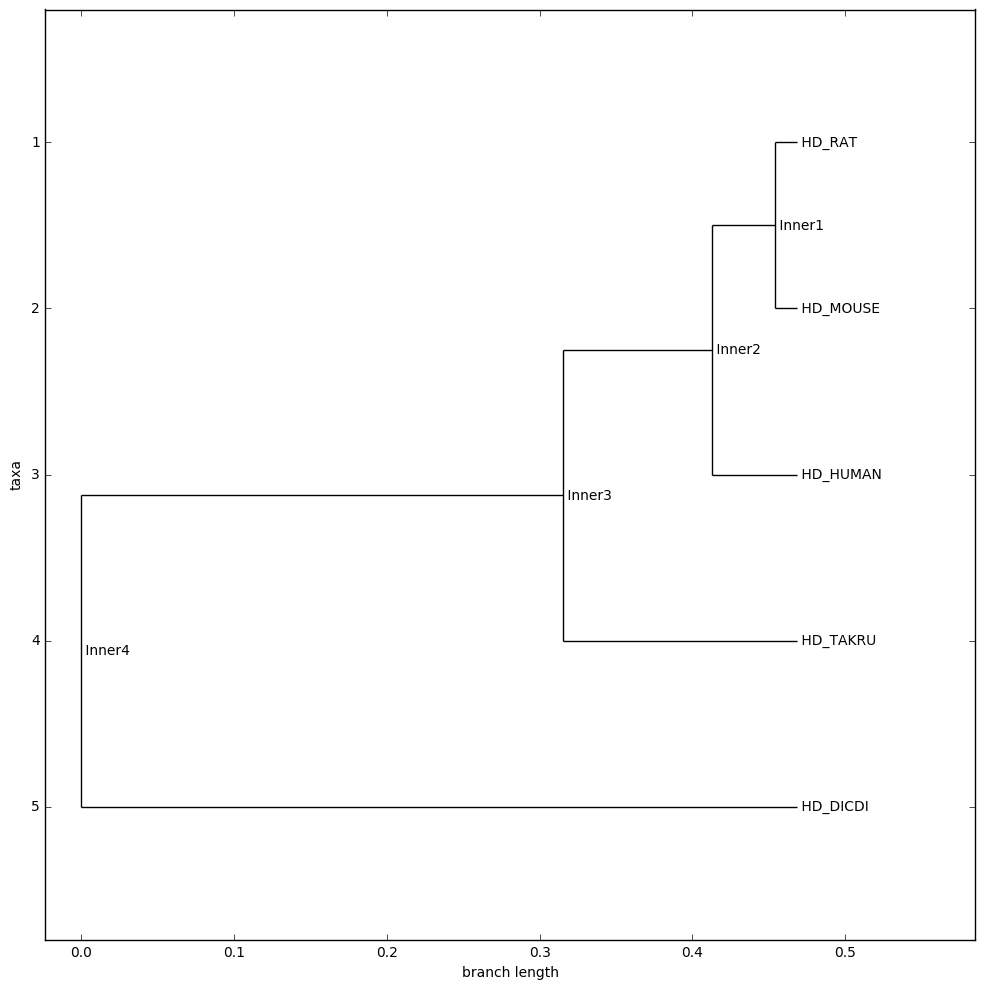
\includegraphics[width=0.8\linewidth]{res/rooted-phylogenetic-tree.png}
    \caption{Rooted phylogenetic tree obtained using the UPGMA algorithm with Jupyter Notebook for protein NP\_002102.4.}
    \label{fig:rooted-phylogenetic-tree}
\end{figure}

% - - - - - - - - - - - - - - - - - - - - - - - - - - -

\subsection{Does it match the BLAST result from Q1/2?}

The orthologues in the obtained phylogenetic tree using UPGMA are:

\textit{Rattus norvegicus}, \textit{Mus musculus}, \textit{Homo sapiens}, \textit{Takifugu rubripes}, and \textit{Dictyostelium discoideum}.

Although I did not focus on them answering the homework, they do match the outputs of my queries. For example, \textit{Rattus norvegicus}, \textit{Mus musculus}, and \textit{Homo sapiens} are listed on section \ref{homologene-results}. And they also show up on the distance tree from question 2. Therefore, yes they do match the results from questions 1 and 2.

\newpage
